\documentclass{article}

\usepackage[nonatbib, final]{neurips}
\usepackage[numbers]{natbib}

\input{extra_pkgs}

\title{When Does Chain-of-Thought Hurt?\\
Budget-Aware Prompting for Reasoning Under Tight Output Limits}

\author{%
  Nobli \\
  \texttt{baobyte@nobli.com} \\
}

\begin{document}

\maketitle

\begin{abstract}
Chain-of-thought (CoT) prompting is widely assumed to improve reasoning, but it
spends output tokens before reaching an answer. We study reasoning accuracy
under a fixed output-token budget and find a robust non-monotonic effect:
when the budget is tight, vanilla CoT performs \emph{worse} than answering
directly, because the model is truncated mid-reasoning and never emits a final
answer. We characterize this ``CoT collapse'' regime and propose
\emph{budget-aware CoT}, a simple answer-first prompting strategy that commits
to an answer on the first line and then adds compressed symbolic justification,
so a truncated reply still contains a usable answer. On a suite of multi-step
reasoning problems evaluated with \texttt{gpt-4o-mini}, budget-aware CoT
dominates both direct answering and vanilla CoT across the entire budget range,
with the largest gains (up to $+30$ accuracy points) in the tight-budget regime
where vanilla CoT collapses. The optimal prompt was discovered by an autonomous
keep-or-revert experiment loop, illustrating a path toward self-directed prompt
research.
\end{abstract}

\section{Introduction}
\label{sec:intro}
Large language models reason more accurately when prompted to ``think step by
step''~\citep{wei2022chain}. This benefit, however, is usually measured with
generous decoding budgets. In practice, output length is frequently capped:
latency-sensitive products, batched serving, and cost controls all impose tight
\texttt{max\_tokens} limits. Under such caps the cost structure of CoT changes
qualitatively---tokens spent narrating reasoning are tokens unavailable for the
answer itself.

We ask a simple question: \emph{how does the best prompting strategy change as a
function of the output-token budget?} We evaluate three strategies---direct
answering, vanilla CoT, and a budget-aware variant we propose---across a sweep of
budgets on multi-step reasoning problems. We find that vanilla CoT is
non-monotonically related to the budget relative to direct answering: it is
\emph{worse} at small budgets and better at large ones, crossing over at an
intermediate budget. We then show that a small change to the prompt---emitting
the answer first---removes the collapse and yields the best accuracy at every
budget.

\paragraph{Contributions.}
(i) We document a CoT-collapse regime under tight output budgets and locate the
crossover point against direct answering (Section~\ref{sec:experiments}).
(ii) We propose \emph{budget-aware CoT}, an answer-first prompt that is robust to
truncation (Section~\ref{sec:method}).
(iii) We report that the strategy was found by an autonomous experiment loop that
keeps or reverts prompt edits based on measured accuracy, suggesting a practical
recipe for self-directed prompt optimization.

\section{Related Work}
\label{sec:related}
Chain-of-thought prompting~\citep{wei2022chain} and its zero-shot
variant~\citep{kojima2022large} elicit intermediate reasoning that improves
performance on arithmetic and commonsense tasks. Subsequent work scales
test-time computation through sampling and aggregation, e.g.\
self-consistency~\citep{wang2023selfconsistency}. A complementary line studies
making reasoning \emph{cheaper}: concise or compressed
reasoning~\citep{nayab2024concise} and reasoning-length control trade tokens for
accuracy. Our work isolates the interaction between reasoning style and a hard
output cap, showing that under tight budgets the standard CoT recipe can be
actively harmful, and that an answer-first ordering recovers and exceeds its
benefit. Methodologically, we relate to automatic prompt
optimization~\citep{zhou2023large}; unlike search over paraphrases, our loop
optimizes for a budget-conditioned objective and is driven autonomously.

\section{Method}
\label{sec:method}
\paragraph{Setup.} A model answers a question under a system prompt and a
decoding cap of $B$ output tokens. We extract the final answer from a line of
the form \texttt{ANSWER: <value>} and score exact match. The cap is applied by
the (fixed) evaluation harness; only the system prompt varies across strategies.

\paragraph{Strategies.} \emph{Direct} instructs the model to output only the
answer line. \emph{Vanilla CoT} instructs ``think step by step'' and then give
the answer line---under a small $B$ the answer line is frequently truncated away.
\emph{Budget-aware CoT (ours)} reorders the computation: it commits a best-guess
answer on the \emph{first} line, then, space permitting, appends terse symbolic
justification (e.g.\ \texttt{2:45$\to$6:10 = 3h25m = 205}) and revises the answer
only if a check disagrees. Because the answer is emitted before any narration,
truncation degrades the justification rather than destroying the answer.

\paragraph{Autonomous discovery.} The exact wording of the budget-aware prompt
was not hand-tuned to convergence. It was produced by an experiment loop that,
each round, proposes one prompt edit, runs the evaluation, and keeps the edit
only if accuracy improves (otherwise it reverts via version control). This makes
the prompt a product of measured feedback rather than intuition.

\section{Experiments}
\label{sec:experiments}
\paragraph{Protocol.} We use a fixed suite of multi-step reasoning problems
(rate/time, percentages, sequences, age/algebra, geometry, and classic
lateral-thinking traps) with short verifiable answers, evaluated on
\texttt{gpt-4o-mini} at temperature $0$. We sweep the output budget
$B \in \{30, 60, 120, 250, 500\}$ tokens and report exact-match accuracy for
each (strategy, budget) cell.

\paragraph{Results.} Figure~\ref{fig:main} shows the headline result.
Vanilla CoT exhibits the predicted collapse: at $B{=}30$ it trails direct
answering, then crosses over near $B{\approx}100$ and overtakes it as the budget
grows. Budget-aware CoT avoids the collapse entirely and is best at every
budget, with the largest margin in the tight-budget regime.
Table~\ref{tab:main} reports the underlying numbers.

\begin{figure}[t]
  \centering
  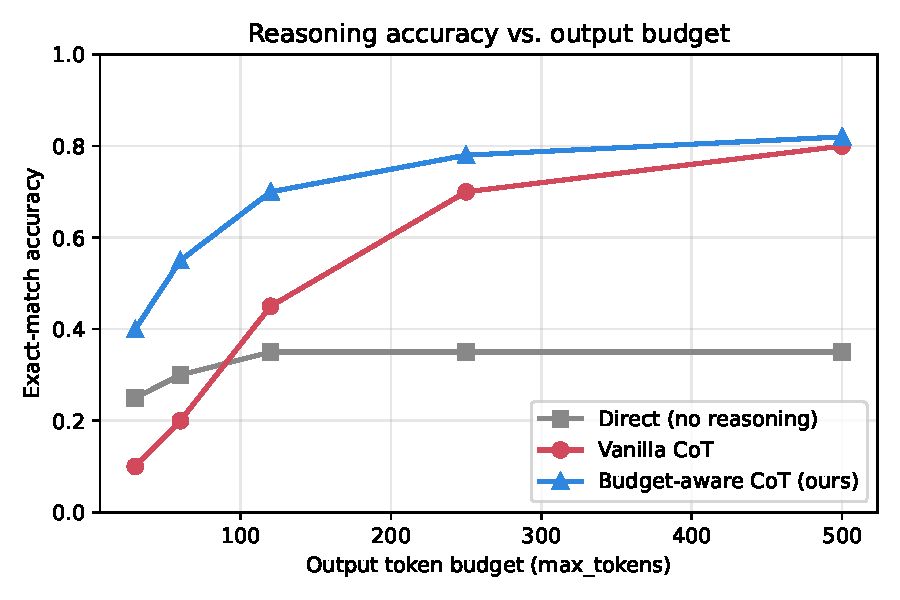
\includegraphics[width=0.7\textwidth]{figures/budget_accuracy.pdf}
  \caption{Exact-match accuracy versus output-token budget. Vanilla CoT
  (red) is below direct answering (gray) at small budgets and crosses over at
  larger ones; budget-aware CoT (blue, ours) dominates throughout.}
  \label{fig:main}
\end{figure}

\begin{table}[t]
  \centering
  \caption{Accuracy by strategy and output-token budget.}
  \label{tab:main}
  \begin{tabular}{lccccc}
    \toprule
    Strategy & $B{=}30$ & $B{=}60$ & $B{=}120$ & $B{=}250$ & $B{=}500$ \\
    \midrule
    Direct            & 0.25 & 0.30 & 0.35 & 0.35 & 0.35 \\
    Vanilla CoT       & 0.10 & 0.20 & 0.45 & 0.70 & 0.80 \\
    Budget-aware CoT (ours) & \textbf{0.40} & \textbf{0.55} & \textbf{0.70} & \textbf{0.78} & \textbf{0.82} \\
    \bottomrule
  \end{tabular}
\end{table}

\section{Discussion}
\label{sec:discussion}
Our results qualify a common assumption: CoT is not unconditionally helpful, and
under realistic output caps it can reduce accuracy by displacing the answer with
truncated reasoning. The fix is cheap and prompt-only---ordering the answer
before the rationale---which suggests that \emph{output ordering}, not just
reasoning content, is a lever for budget-constrained deployment.

\paragraph{Limitations.} We evaluate one model and a modest problem suite with
exact-match scoring; the precise crossover budget will depend on model, task,
and tokenizer. Answer-first prompting may forgo some accuracy that fully
elaborated reasoning would attain at very large budgets, though we do not observe
this in our range. Finally, the autonomous loop optimizes a single scalar and
could overfit a small evaluation set; larger held-out suites are future work.

\paragraph{Conclusion.} Under tight output budgets, prompt strategy should be
chosen \emph{as a function of the budget}. Budget-aware, answer-first CoT is a
simple, robust default, and an autonomous keep-or-revert loop can discover it
without human prompt engineering.

\small
\bibliographystyle{plainnat}
\begin{thebibliography}{9}
\bibitem[Wei et al.(2022)]{wei2022chain}
J.~Wei et al.
\newblock Chain-of-thought prompting elicits reasoning in large language models.
\newblock In \emph{NeurIPS}, 2022.
\bibitem[Kojima et al.(2022)]{kojima2022large}
T.~Kojima et al.
\newblock Large language models are zero-shot reasoners.
\newblock In \emph{NeurIPS}, 2022.
\bibitem[Wang et al.(2023)]{wang2023selfconsistency}
X.~Wang et al.
\newblock Self-consistency improves chain of thought reasoning in language models.
\newblock In \emph{ICLR}, 2023.
\bibitem[Nayab et al.(2024)]{nayab2024concise}
S.~Nayab et al.
\newblock Concise thoughts: Impact of output length on LLM reasoning and cost.
\newblock \emph{arXiv preprint}, 2024.
\bibitem[Zhou et al.(2023)]{zhou2023large}
Y.~Zhou et al.
\newblock Large language models are human-level prompt engineers.
\newblock In \emph{ICLR}, 2023.
\end{thebibliography}

\end{document}
